\chapter{Power Train controller}
The power train controller consists in two units. The actual controller CU-320-2DP and power unit, a frequency inverter of single motor module, model 6SL3126-1TE28-5AA0 of cold plate type. Additionally is installed a CBC10 CAN controller adaptor inside CU-320DP that allow the communication via CAN bus.

In figure \ref{fig:siemens_cu320_module} and \ref{fig:siemens_motor_module} are presented the controller board and frequency inverter with respective diagrams.
The connections between each Siemens modules are made via a crossover ethernet cable using one of its Drive-CLiQ ports. The electronics power source requires 24V \gls{DC}, that should be supplied for both modules using the auxiliary battery pack which can be  cut using the emergency button.


To connect CU-320DP to \href{https://w3.siemens.com/mcms/mc-solutions/en/engineering-software/starter-commissioning-tool/pages/starter-commissioning-tool.aspx}{Siemens Starter software}, is also necessary to use a crossover cable connected to the respective LAN configuration port (see figure \ref{fig:siemens_cu320_module}). 

Each module has a few leds to visually transmit the current status of device. Table \ref{tab:CU320_led_status} and \ref{tab:motor_led_status} describe status of CU-320-DP and frequency inverter module respective.

\begin{figure}
	\centering
	\subcaptionbox{Controller module mounted on car.}{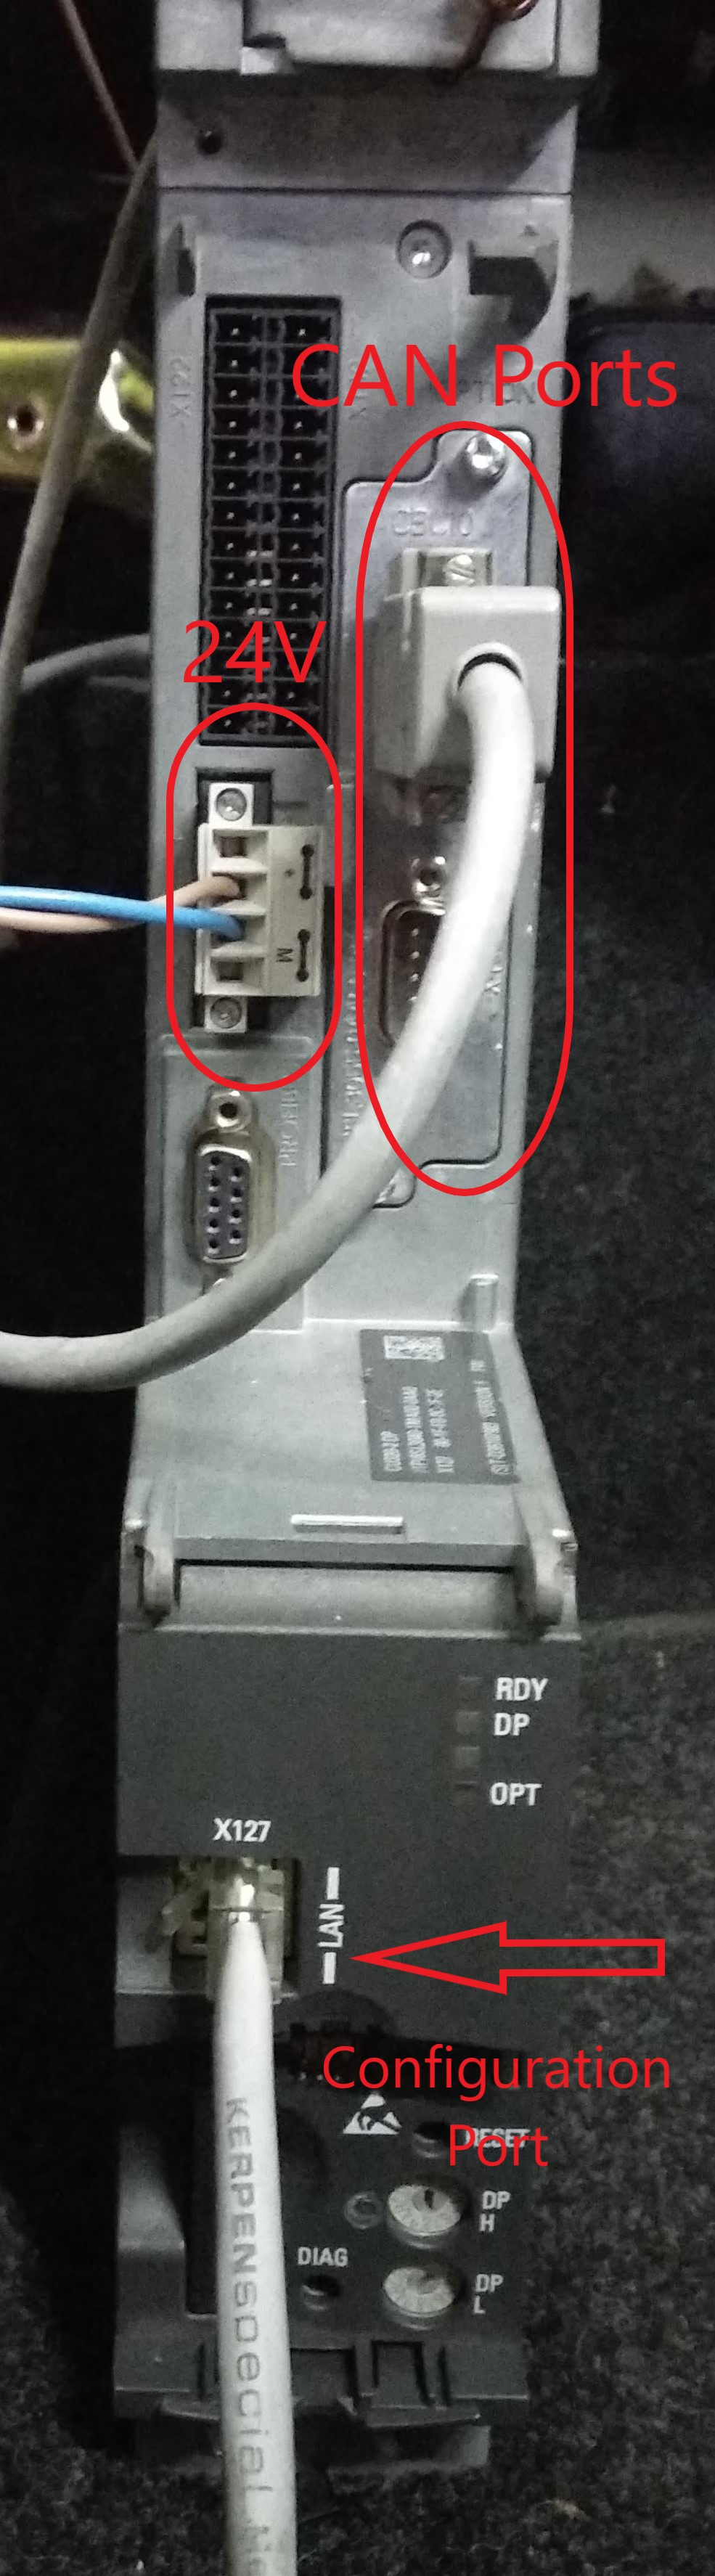
\includegraphics[width=0.2\linewidth]{figures/siemens_CU320DP}}
	\subcaptionbox{Generic diagram (source \cite{siemens_equipment_control})}{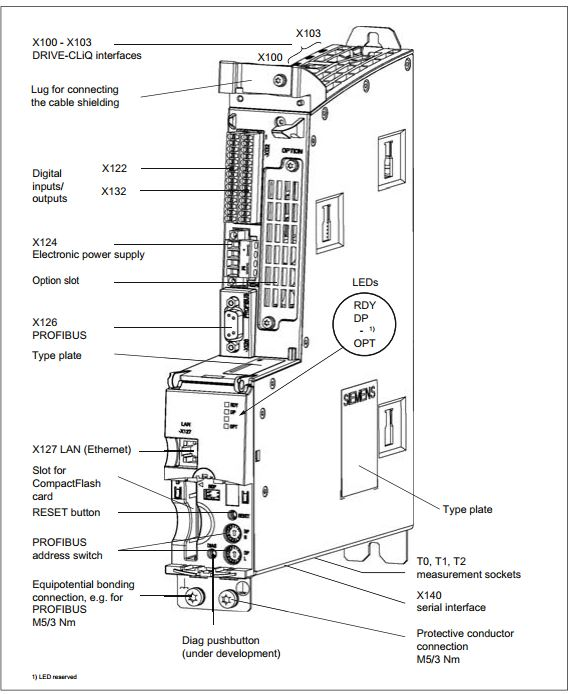
\includegraphics[width=0.6\linewidth]{figures/siemens_CU320DP_diagram}}
	\caption{Siemens CU320-2DP module}
	\label{fig:siemens_cu320_module}
\end{figure}

\begin{figure}
	\centering
	\subcaptionbox{Motor module mounted on car.}{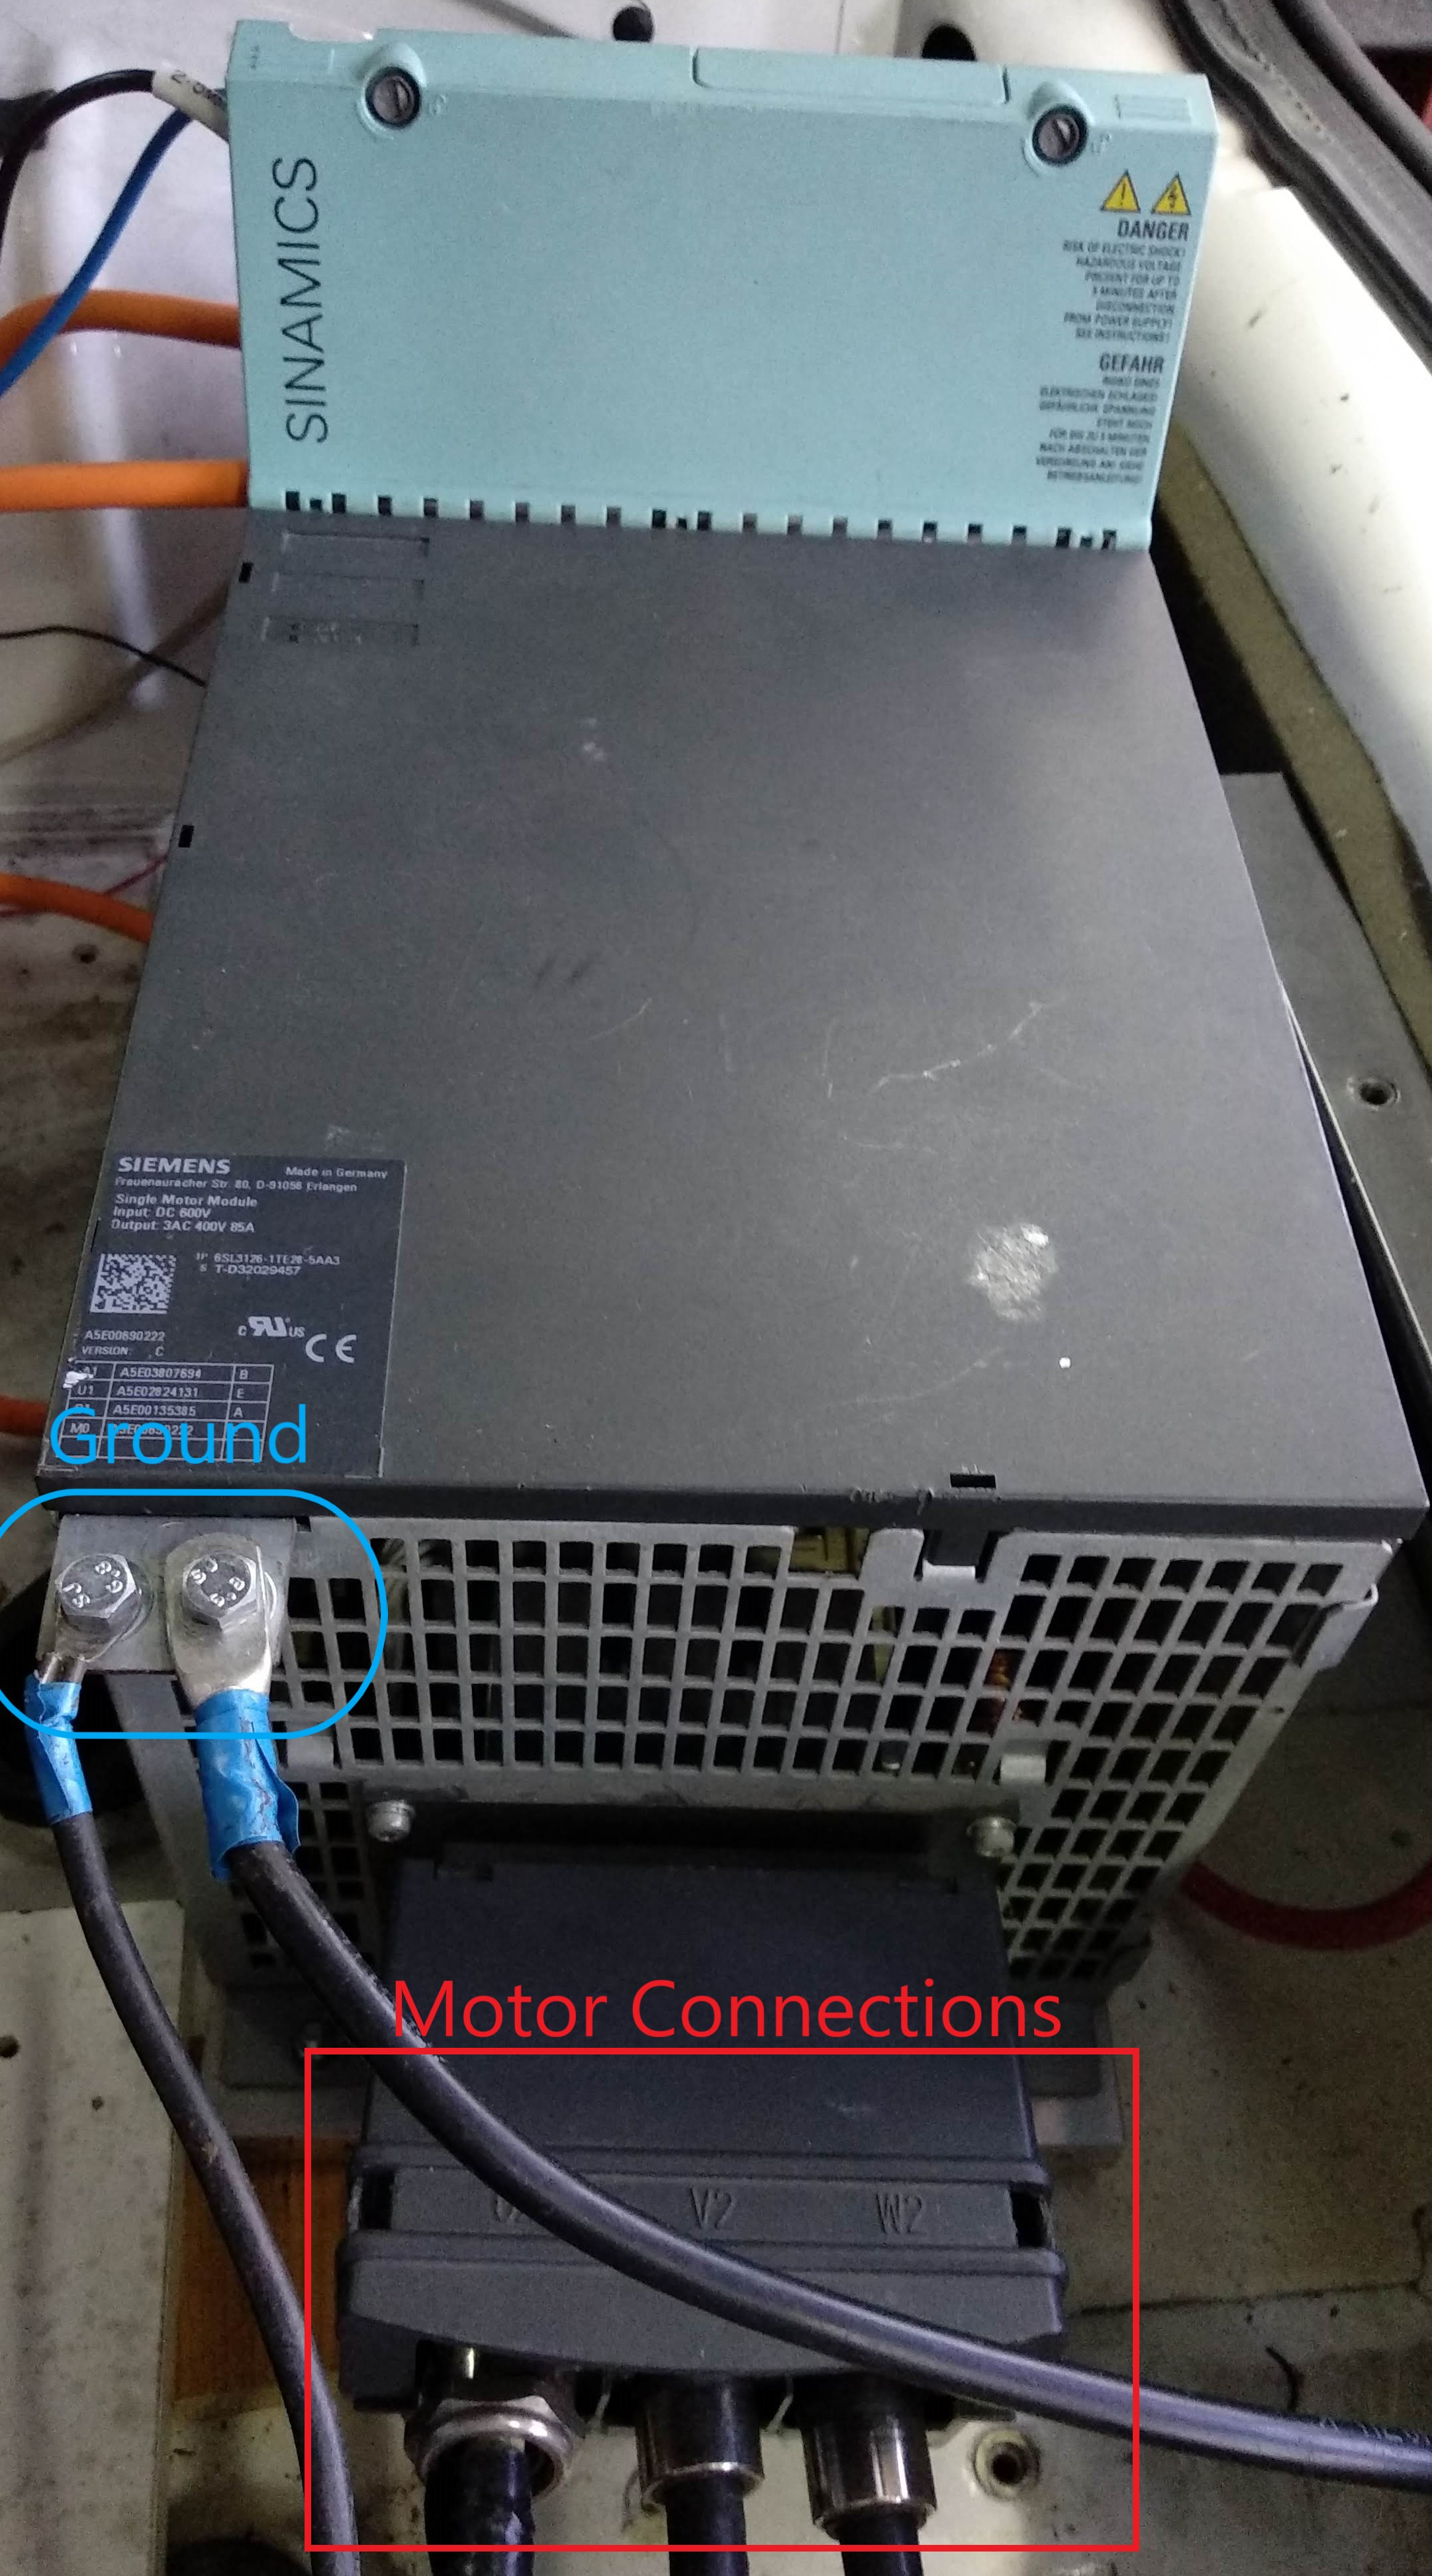
\includegraphics[width=0.3\linewidth]{figures/siemens_motor_module}}
	\subcaptionbox{Generic diagram (source \cite{siemens_equipment})}{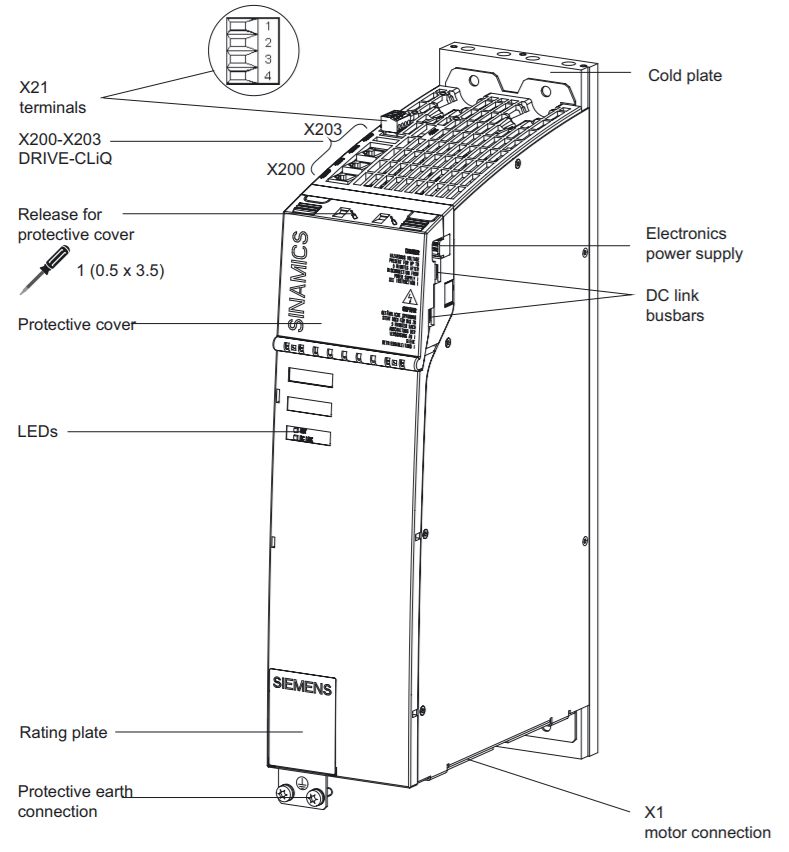
\includegraphics[width=0.5\linewidth]{figures/siemens_motor_module_diagram}}
	\caption{Siemens motor module - frequency inverter}
	\label{fig:siemens_motor_module}
\end{figure}

\begin{table}[!hb]
	\centering
	\baselinestretch{1.5}
	\begin{tabular}{ccM{0.15\linewidth}M{0.5\linewidth}}
		\toprule
		\textbf{LED} & \textbf{Color} & \textbf{State} & \textbf{Description}\\
		\midrule
		\multirow{9}{*}{Ready} & - & OFF & Electronics power supply outside permissible tolerance range. \\
		\cmidrule{2-4}
		&\multirow{3}{*}{Green} & Continuous & The component is ready for operation and cyclic DRIVE-CLiQ
		communication is taking place.\\
		& & Flashing 0.5Hz & Commissioning/reset\\
		& & Flashing 2Hz & Writing to the memory card\\
		\cmidrule{2-4}
		&Orange & Continuous & DRIVE-CLiQ communication is being established.\\
		\cmidrule{2-4}
		& Red & Continuous & At least one fault is present in this component.\\
		\cmidrule{2-4}
		&Green/Red & Flashing 2Hz & Firmware is being downloaded\\
		\cmidrule{2-4}
		&Green/Orange & Flashing 2Hz 
& Component recognition via LED is activated (p0124).\\
		\midrule
		\multirow{3}{*}{DC Link} & - & OFF & Electronics power supply outside permissible tolerance range.\\
		& Orange & Continuous & DC link voltage within permissible tolerance range\\
		& Red & Continuous & DC link voltage outside permissible tolerance range\\
		\midrule
		\multirow{7}{*}{OPT} &  - & OFF & Board not installed.\\
		\cmidrule{2-4}
		& \multirow{3}{*}{Green} & Continuous & NMT Operational.\\
		& & Flashing 2.5Hz & NMT Preoperational.\\
		& & Single flash & Stopped.\\
		\cmidrule{2-4}
		& \multirow{3}{*}{Red} & Continuous & BUS off.\\
		& & Single flash & Error Passive Mode.\\ 
		& & Double flash & Error Control Event, a Life-Guard Event has occurred .\\
		\bottomrule
	\end{tabular}
	\caption{Siemens control unit module led status}
	\label{tab:CU320_led_status}
\end{table}

\begin{table}[!hb]
	\centering
	\begin{tabular}{ c c M{0.15\linewidth} M{0.5\linewidth}}
		\toprule
		\textbf{LED} & \textbf{Color} & \textbf{State} & \textbf{Description}\\
		\midrule
		\multirow{6}{*}{\vspace{-1.5cm} Ready} & - & OFF & Electronics power supply outside permissible tolerance range. \\
		\cmidrule{2-4}% That's the rule you're looking for.
		&Green & Continuous & The component is ready for operation and cyclic DRIVE-CLiQ
		communication is taking place.\\
		\cmidrule{2-4}% That's the rule you're looking for.
		&Orange & Continuous & DRIVE-CLiQ communication is being established.\\
		\cmidrule{2-4}% That's the rule you're looking for.
		& Red & Continuous & At least one fault is present in this component.\\
		\cmidrule{2-4}% That's the rule you're looking for.
		&Green/Red & Flashing 2Hz & Firmware is being downloaded\\
		\cmidrule{2-4}% That's the rule you're looking for.
		&Green/Orange & Flashing 2Hz 
& Component recognition via LED is activated (p0124).\\
		\midrule
		\multirow{3}{*}{\vspace{-0.5cm} DC Link} & - & OFF & Electronics power supply outside permissible tolerance range.\\
		\cmidrule{2-4}% That's the rule you're looking for.
		& Orange & Continuous & DC link voltage within permissible tolerance range\\
		\cmidrule{2-4}% That's the rule you're looking for.
		& Red & Continuous & DC link voltage outside permissible tolerance range\\
		\bottomrule
	\end{tabular}
	\caption{Siemens Motor module led status}
	\label{tab:motor_led_status}
\end{table}
 
\begin{table}
	\centering
	\begin{tabular}{lcc}
		\toprule
		\textbf{Parameter} & \textbf{Value} & \textbf{Units}\\
		\midrule
		Weight & 1200 & kg\\
		Batteries Weight & 400 & kg\\
		Autonomy & 90 & km \\
		Maximum speed & 100 & km/h \\
		Acceleration (0-50km/h) & 8 & s \\
		Wheel diameter & 60.97 & cm \\
		Width & 150.8 & cm \\
		Height & 144.5 & cm \\
		Area & 2.18 & $\text{m}^2$ \\
		Drag Coefficient & 0.33 & - \\
		\bottomrule
	\end{tabular}
	\caption{Original car parameters}
	\label{tab:car_parameters}
\end{table}



\section{Motor data}

The motor data extracted from motor plate and manual of the car are presented in table \ref{tab:motor_parameters}. These values are essential to describe the motor inside the commissioning software, Siemens Starter. Information about the nominal operation points of the motor are also described in table \ref{tab:motor_nameplate_data}. Although currently is not required, for future reference, in table \ref{tab:car_parameters} is also present the original car parameters extracted from manufacture manual.
 

\begin{table}
	\centering
	\begin{tabular}{lcc}
		\toprule
		\textbf{Parameter} & \textbf{Value} & \textbf{Units}\\
		\midrule
		Maximum Power & 30 & kW\\  
		Maximum Torque & 130 & Nm \\
		Maximum speed & 10000 & rpm \\
		Weight & 41.5 & kg \\
		Power factor & 0.85 & --\\
		\midrule
		\multicolumn{3}{c}{\textbf{Equivalent circuit parameters}}\\
		\midrule
		stator resistance & 8.56 & mOhms \\
		stator leakage inductance & 0.06292 & mH \\
		Iron Resistance & $\infty$ & mOhms\\
		Mutual Inductance & 1.0122 & mH \\
		rotor resistance & 5.10 & mOhms \\
		rotor leakage inductance & 0.06709 & mH \\
		\bottomrule
	\end{tabular}
	\caption{Motor parameters}
	\label{tab:motor_parameters}
\end{table}

\begin{table}
	\centering
	\begin{tabular}{ccccc}
		\toprule
		\textbf{U (V)} & \textbf{f (Hz)} & \textbf{I (A)} & \textbf{Torque (Nm)} & \textbf{Speed (rpm)} \\
		\midrule
		76 & 76 & 157 & 65 & 2200 \\
		121 & 220 & 90 & 22 & 6500 \\
		121 & 305 & 88 & 16 & 9000 \\
		\bottomrule
	\end{tabular}
	\caption{Motor Nameplate parameters}
\label{tab:motor_nameplate_data}
\end{table}



\section{Siemens Starter}

Starter is the software available from Siemens used to configure the all Siemens modules. This configuration should only be required at the beginning or if it is wanted to make structural changes from current project. The project is then saved to memory card and should load every time the power is applied. Next will be described the procedure to achieve the current status stored in the memory card. The base configuration follows the instructions from \cite{siemens_comissioning_manual} chapter 3.4, which user must follow, and only the changes from default values are presented to achieve the current status. Follow the Starter setup wizard step by step and choose to find unities online while ensuring the PC is connected via crossover cable to control unit, selecting the respective ethernet interface. It is also possible to configure all in offline mode, if no physical connection available at the moment.
In figure \ref{fig:starter_config} are presented the principal elements to serve as example for user.

\begin{description}[align=left, labelwidth=10em, leftmargin=5em, style=nextline]
	\item[CAN Module CBC10] The choosen \textbf{node ID} is \textbf{2}. The speed is \textbf{1Mbit/s}. Select standard PDO Mapping of 4 Receive and 4 transmit.
	\vspace{1ex}
	\begin{mdframed}[backgroundcolor=red!20, roundcorner=10pt, innertopmargin=5pt, innerbottommargin=5pt, skipabove=0pt]
		\Warning \, \textbf{Caution! The CBC10 is not terminated and is working in ground-free operation. The termination is active in the \gls{EPOS} device which shares the same CAN bus line. Check \cite{siemens_comissioning_manual} to change it.}
	\end{mdframed}
	%-------------------------------------------------------------------------------
	\item[Motor configuration:] Select control type \textbf{[20] speed control (encoderless)}. In voltage select \textbf{510 to 720 VDC}. In power section module select \textbf{Cold Plated}, \textbf{Single motor modules} and from the list choose \textbf{6SL3126-1TE28-5Axx}, the module with 45.6kW 85A. In the next section, place infeed operation with 1. Select enter motor data, induction motor and use tables \ref{tab:motor_parameters} and \ref{tab:motor_nameplate_data} for entering the the requested information.
	%---------------------------------------------------------------------------------
	\item[Enable CAN access to motor drive] On expert list of CU320-2DP enable CAN acess to motor drive registers by changing \textbf{p8630[0]} to 2.
	%---------------------------------------------------------------------------------
	\item[CAN interconnect] To accept reference and commands from CAN interface performe the following list of changes to expert list registers of motor module:
	\begin{description}
		\item[p0840{[0]}] ON / OFF (OFF1) set to CAN control word bit 0 meaning register r8890.0
		\item[p0844{[0]}] No coast-down / coast-down (OFF2) signal source set to CAN control word bit 1 meaning register r8890.1
		\item[p0848{[0]}] No Quick Stop / Quick Stop (OFF3) signal source set to CAN control word bit 2 meaning register r8890.2.
		\item[p0852{[0]}] Enable operation/inhibit operation set to CAN control word bit 3 meaning register r8890.3.
		\item[p864] Infeed operation set it to 1.
		\item[p1070{[0]}] set main setpoint to default PDO2 second variable, speed by selecting r8860[1] IF2 PDZ Receive double word PDZ 2+3.
		\item[p1122{[0]}]] Bypass ramp-function generator set it to 1.
		\item[p1317{[0]}] U/f control activation set to active.
		\item[p2103{[0]}] 1st acknowledge faults set to CAN control word bit 1 meaning register r8890.7.
		\item[p8744] CAN PDO mapping configuration set it to [1] Predefined Connection Set. This setting will use activate the default PDO settings for CANOpen. Check if configuration is correct by inspecting the following registers presented on table \ref{tab:default_PDO}.
		\item[p8851{[0]}] IF2 PZD send word PZD 1 to status word, meaning r8784.
		\item[p8851{[3]}] IF2 PZD send word PZD 4 to torque actual value, meaning r80.
		\item[p8861{[1]}] IF2 PZD send double word PZD 2 + 3 to actual speed smoothed, meaning r63.
		\item[p10] Set to ready after all configuration settings.
	\end{description}
\end{description}

\begin{table}[!h]
	\centering
	\begin{tabular}{lll}
		\toprule
		\textbf{Register} & Description & Value\\
		\midrule
		p8700[0] & CAN Receive PDO 1, PDO COB-ID & 202H \\ 
		p8701[0] & CAN Receive PDO 2, PDO COB-ID & 302H \\
		p8702[0] & CAN Receive PDO 3, PDO COB-ID & 402H \\
		p8703[0] & CAN Receive PDO 4, PDO COB-ID & 502H \\
		\midrule
		p8710[0] & CAN Receive Mapping for RPDO 1, Mapped object 1 & 60400010H \\
		p8711[0] & CAN Receive Mapping for RPDO 2, Mapped object 1 & 60400010H \\
		p8711[1] & CAN Receive Mapping for RPDO 2, Mapped object 2 & 60FF0020H \\
		p8712[0] & CAN Receive Mapping for RPDO 3, Mapped object 1 & 60400010H \\
		p8712[1] & CAN Receive Mapping for RPDO 3, Mapped object 2 & 60710010H \\
		p8713[0] & CAN Receive Mapping for RPDO 4, Mapped object 1 & 60400010H \\
		p8713[1] & CAN Receive Mapping for RPDO 4, Mapped object 2 & 60FF0020H \\
		p8713[2] & CAN Receive Mapping for RPDO 4, Mapped object 3 & 60710010H \\
		\midrule
		p8720[0] & CAN Transmit PDO 1, PDO COB-ID & 40000182H \\
		p8721[0] & CAN Transmit PDO 2, PDO COB-ID & 40000282H \\
		p8722[0] & CAN Transmit PDO 3, PDO COB-ID & 40000382H \\
		p8723[0] & CAN Transmit PDO 4, PDO COB-ID & 40000482H \\
		\midrule
		p8730[0] & CAN Transmit Mapping for TPDO 1, Mapped object 1 & 60410010H \\
		p8731[0] & CAN Transmit Mapping for TPDO 2, Mapped object 1 & 60410010H \\
		p8731[1] & CAN Transmit Mapping for TPDO 2, Mapped object 2 & 606C0020H \\
		p8732[0] & CAN Transmit Mapping for TPDO 3, Mapped object 1 & 60410010H \\
		p8732[1] & CAN Transmit Mapping for TPDO 3, Mapped object 2 & 60740010H \\
		p8733[0] & CAN Transmit Mapping for TPDO 4, Mapped object 1 & 60410010H \\
		p8733[1] & CAN Transmit Mapping for TPDO 4, Mapped object 2 & 60630020H \\
	\end{tabular}
	\caption{Default values of CANOpen PDO configuration (assuming node ID = 2 )}
	\label{tab:default_PDO}
\end{table}

\begin{figure}
	\centering
	\begin{subfigure}{0.45\linewidth}
		\centering
		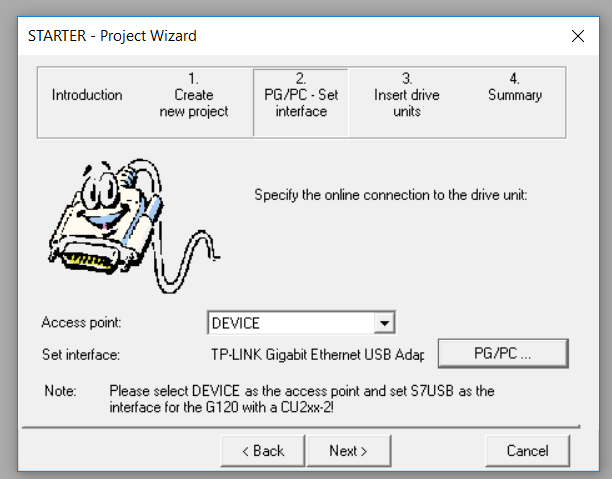
\includegraphics[width=0.7\linewidth]{figures/starter_01}
		\caption{PC interface selection}
	\end{subfigure}
	\begin{subfigure}{0.45\linewidth}
		\centering
		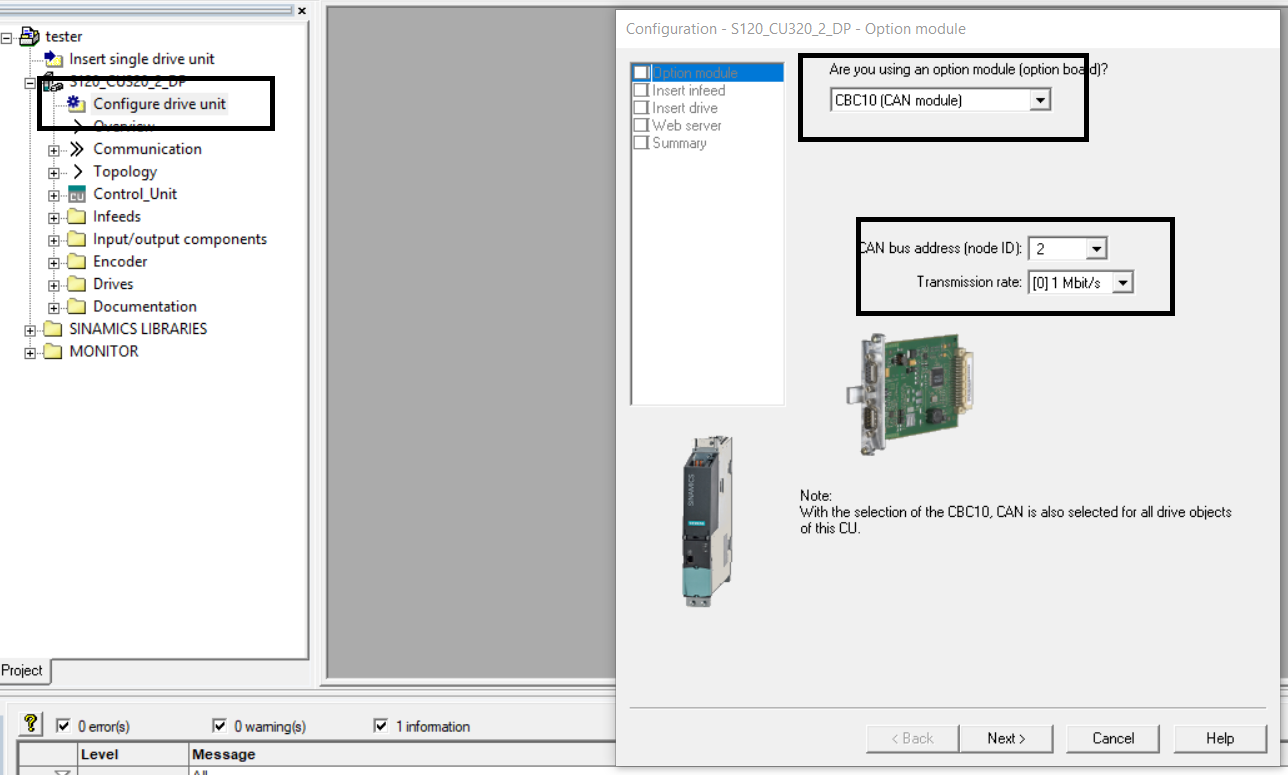
\includegraphics[width=0.9\linewidth]{figures/starter_02}
		\caption{CAN module configuration}
	\end{subfigure}
	\\
	\vspace{1cm}
	\begin{subfigure}{0.32\linewidth}
		\centering
		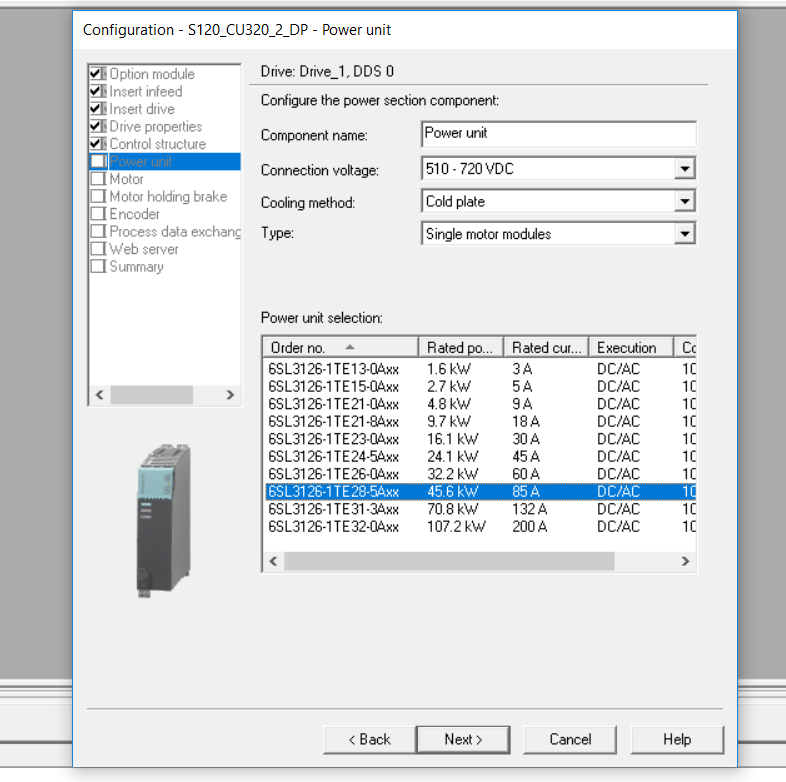
\includegraphics[width=0.9\linewidth]{figures/starter_03}
		\caption{Motor module selection}
	\end{subfigure}
	\hfill
	\begin{subfigure}{0.32\linewidth}
		\centering
		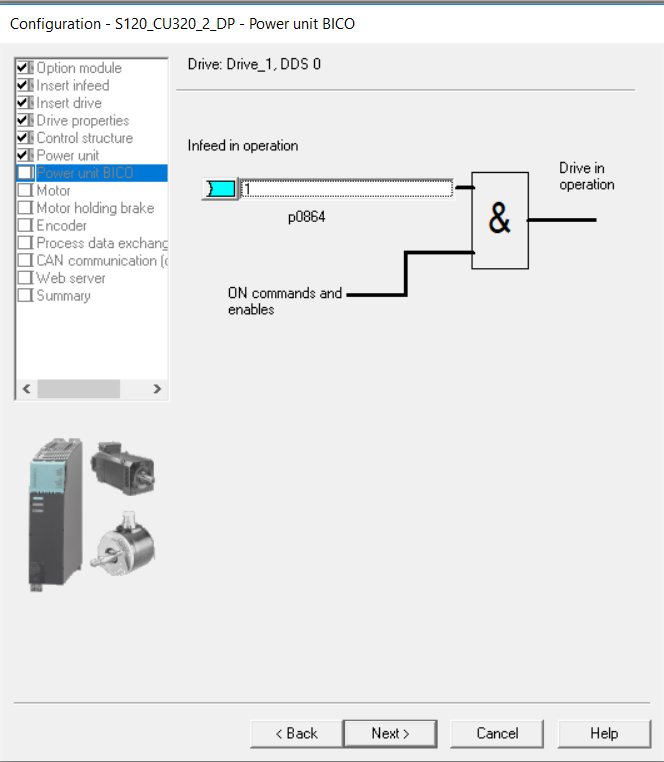
\includegraphics[width=0.8\linewidth]{figures/starter_04}
		\caption{Infeed setting}
	\end{subfigure}
	\hfill
	\begin{subfigure}{0.32\linewidth}
		\centering
		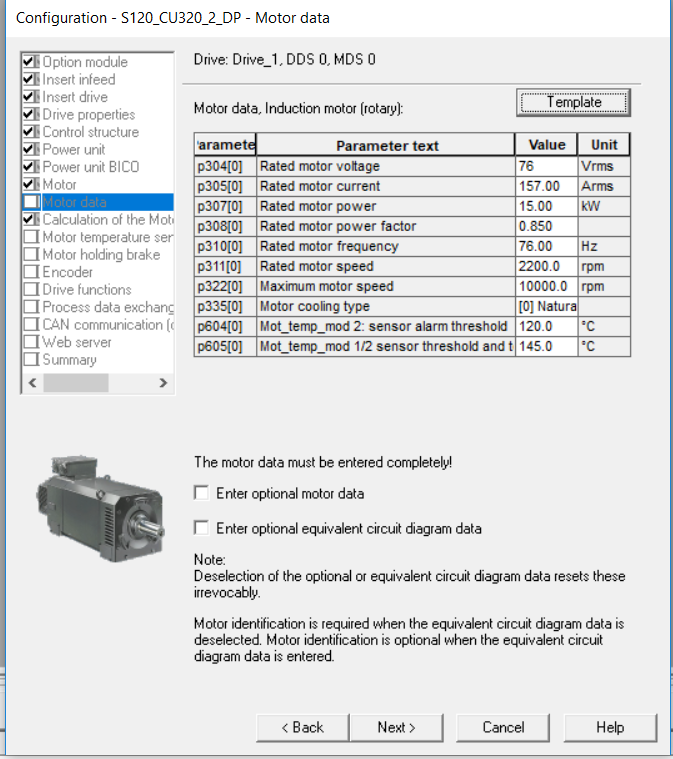
\includegraphics[width=0.8\linewidth]{figures/starter_05}
		\caption{Motor data}
	\end{subfigure}
\caption{Main points of starter configuration wizard}
\label{fig:starter_config}
\end{figure}

\section{Interface library}

The developed interface library for Sinamics devices is present in appendix \ref{appendix:sinamics}. The library is written in python language and using the CAN interface to interact with CU320-2DP. User should note that the library still not cover all the possible interactions and modes of operation. It is only designed for speed control without encoder. Similar to other code presented in this report, user should always prefer the online documentation to grant is the most updated version, that is in the Github repository.